\documentclass[12pt, a4paper, brazil]{article}
\usepackage[brazil]{babel}
\usepackage[utf8]{inputenc}
\usepackage[T1]{fontenc}
\usepackage{graphicx}
\usepackage{indentfirst}
\usepackage{hyperref}
\usepackage{url}
\urlstyle{same}

\usepackage{natbib}
\bibliographystyle{plain}

\title{Comparação dos Resultados de Algoritmos de Classificação}
\author{Augusto Ribas$^1$, Bruno Nazário$^1$ e Doglas Sorgatto$^1$}
\date{$^1$Faculdade de Computação - Universidade Federal de Mato Grosso do Sul}

\begin{document}

\maketitle

\begin{abstract}
Avaliamos o desempenho de três algoritmos de classificação: o KNN (K-nearest neighbors), a árvore de decisão e o Naive Bayes;
\end{abstract}
%
\section{Introdução}

Exemplo de citação  \citep{Mitchell1997}

\subsection{Problema}
ghhjghfghf

\subsection{Objetivos}
kjfdfhdjfhdjff

\section{Material e Métodos}

\subsection{Algoritmos de Classificação}
kjdffkdjf
\subsubsection{Vizinhos mais próximos}
fdkfdkfjdj
\subsubsection{Arvore de Decisão}
fdfdjfhjhdf
\subsubsection{Naive Bayes}
jfdkjfdkjfdjf

\subsection{Procedimentos gerais}
O que foi feito na organização do algoritmo, como se deu a separação em folds, etc.

\subsection{Conjuntos de dados}

Foram utilizados 10 conjuntos de dados.

\subsubsection{Iris}
Este é talvez o conjunto de dados mais comum em estudos de reconhecimento de padrões na literatura, usado pela primeira vez pelo famoso biólogo evolucionista Ronald Aylmer Fisher \citep{Fisher1936}. O conjunto de dados contém 3 classes com 50 exemplos de cada classe e com quatro atributos por exemplo, o tamanho e largura de pétalas e sépalas, onde cada classe é uma espécie vegetal do gênero \emph{Iris}.

O dataset Iris pode ser obtido no endereço \url{https://archive.ics.uci.edu/ml/datasets/Iris} e suas informações básicas são:
\begin{table}[!ht]
\centering
\caption{Iris Data Set}
\label{iristable}
\begin{tabular}{|l|l|}
\hline
Característica & Multivariável\\
\hline
Tipo dados & real\\
\hline
Instâncias & 150\\
\hline
Atributos & 4 \\
\hline
\end{tabular}
\end{table}

\subsubsection{Ecoli}
O dataset Ecoli pode ser obtido no endereço \url{https://archive.ics.uci.edu/ml/datasets/Ecoli} e suas informações básicas são:
\begin{table}[!ht]
\centering
\caption{Ecoli Data Set}
\label{ecolitable}
\begin{tabular}{|l|l|}
\hline
Característica & Multivariável\\
\hline
Tipo dados & real\\
\hline
Instâncias & 336\\
\hline
Atributos & 8 \\
\hline
\end{tabular}
\end{table}

\subsubsection{Fertility}
O dataset Fertility pode ser obtido no endereço \url{https://archive.ics.uci.edu/ml/datasets/Fertility} e suas informações básicas são:
\begin{table}[!ht]
\centering
\caption{Fertility Data Set}
\label{fertilitytable}
\begin{tabular}{|l|l|}
\hline
Característica & Multivariável\\
\hline
Tipo dados & real\\
\hline
Instâncias & 100\\
\hline
Atributos & 10 \\
\hline
\end{tabular}
\end{table}

\subsubsection{Yeast}
O dataset Yeast pode ser obtido no endereço \url{https://archive.ics.uci.edu/ml/datasets/Yeast} e suas informações básicas são:
\begin{table}[!ht]
\centering
\caption{Yeast Data Set}
\label{yeasttable}
\begin{tabular}{|l|l|}
\hline
Característica & Multivariável\\
\hline
Tipo dados & real\\
\hline
Instâncias & 1484\\
\hline
Atributos & 8\\
\hline
\end{tabular}
\end{table}

\subsubsection{Planning Relax}
O dataset Planning Relax pode ser obtido no endereço \url{https://archive.ics.uci.edu/ml/datasets/Planning+Relax} e suas informações básicas são:
\begin{table}[!ht]
\centering
\caption{Planning Relax Data Set}
\label{planningtable}
\begin{tabular}{|l|l|}
\hline
Característica & Multivariável\\
\hline
Tipo dados & real\\
\hline
Instâncias & 182\\
\hline
Atributos & 13\\
\hline
\end{tabular}
\end{table}

\subsubsection{Habermans Survival}
O dataset Haberman's Survival pode ser obtido no endereço \url{https://archive.ics.uci.edu/ml/datasets/Haberman's+Survival} e suas informações básicas são:
\begin{table}[!ht]
\centering
\caption{Haberman's Survival Data Set}
\label{habermanstable}
\begin{tabular}{|l|l|}
\hline
Característica & Multivariável\\
\hline
Tipo dados & inteiro\\
\hline
Instâncias & 306\\
\hline
Atributos & 3\\
\hline
\end{tabular}
\end{table}

\subsubsection{banknote authentication}
O dataset Banknote Authentication pode ser obtido no endereço \url{https://archive.ics.uci.edu/ml/datasets/banknote+authentication} e suas informações básicas são:
\begin{table}[!ht]
\centering
\caption{Banknote Authentication Data Set}
\label{banknotetable}
\begin{tabular}{|l|l|}
\hline
Característica & Multivariável\\
\hline
Tipo dados & real\\
\hline
Instâncias & 1372\\
\hline
Atributos & 5\\
\hline
\end{tabular}
\end{table}

\subsubsection{Breast Cancer Wisconsin}
O dataset Breast Cancer Wisconsin pode ser obtido no endereço \url{https://archive.ics.uci.edu/ml/datasets/Breast+Cancer+Wisconsin+(Original)} e suas informações básicas são:
\begin{table}[!ht]
\centering
\caption{Breast Cancer Wisconsin Data Set}
\label{breasttable}
\begin{tabular}{|l|l|}
\hline
Característica & Multivariável\\
\hline
Tipo dados & inteiro \\
\hline
Instâncias & 699 \\
\hline
Atributos & 10\\
\hline
\end{tabular}
\end{table}

\subsubsection{Mammographic Mass}
O dataset Mammographic Mass pode ser obtido no endereço \url{https://archive.ics.uci.edu/ml/datasets/Mammographic+Mass} e suas informações básicas são:
\begin{table}[!ht]
\centering
\caption{Mammographic Mass Data Set}
\label{mammographictable}
\begin{tabular}{|l|l|}
\hline
Característica & Multivariável\\
\hline
Tipo dados & inteiro \\
\hline
Instâncias & 961 \\
\hline
Atributos & 6\\
\hline
\end{tabular}
\end{table}

\subsubsection{Pima Indians Diabetes}
O dataset Pima Indians Diabetes pode ser obtido no endereço \url{https://archive.ics.uci.edu/ml/datasets/Pima+Indians+Diabetes} e suas informações básicas são:
\begin{table}[!ht]
\centering
\caption{Pima Indians Diabetes Data Set}
\label{pimatable}
\begin{tabular}{|l|l|}
\hline
Característica & Multivariável\\
\hline
Tipo dados & inteiro e Real \\
\hline
Instâncias & 768 \\
\hline
Atributos & 8\\
\hline
\end{tabular}
\end{table}

\section{Resultados e Discussão}

\begin{figure}[!htb]
  \caption{Comparação das acurácias para os três métodos de classificação}
  \centering
%    \includegraphics[width=0.5\textwidth]{Iris/acuracias.png}
\end{figure}

\begin{figure}[!htb]
  \caption{Escolha do número de vizinhos mais próximos}
  \centering
%    \includegraphics[width=0.5\textwidth]{Iris/knn.png}
\end{figure}

\begin{figure}[!htb]
  \caption{Árvore de decisão gerada}
  \centering
%    \includegraphics[width=0.5\textwidth]{Iris/arvore.eps}
\end{figure}

\section{Considerações Finais}
O que aprendemos com o trabalho
\newpage
\bibliography{Trabalho_IA.bib}

\end{document}
